\section{Spracovanie záverečnej práce}

\subsection{Písanie odborného textu}

Pri písaní záverečných prác je vhodné dodržiavať nasledovné zásady písania odborného textu: 

\begin{itemize}
	\item V odbornom texte sa využívajú štylistické prostriedky, ktoré sa vyhýbajú opakovanému použitiu slova ja. Jedným je užívanie autorského alebo tiež skromného plurálu, ktorý je obvyklý v definičných procesoch (Ako objekt označujeme,..). Neosobné vyjadrovanie vyjadríme aj použitím pasívnych konštrukcií (Tretia kapitola je doplnená.., boli popísané,…).
	\item Zo slovných spojení sa v odbornom texte objavujú spojenia, ktoré odkazujú:
	\begin{itemize}
		\item miestne: vyššie / nižšie uvádzame, v nasledujúcej kapitole,..
		\item časovo: doteraz sme pojednávali .., skôr než pristúpime k výkladu…
		\item procesuálne: ak sa vrátime k funkcii.., zakončili sme ..
	\end{itemize}
	\item Myšlienky vlastné sú oddeľované od myšlienok prevzatých, ktoré citujeme
\end{itemize}

\subsubsection{Interpunkčné znamienka}

\paragraph{Spojovník a pomlčka}

Spojovník sa píše pomocou rozdeľovacieho znamienka bez medzier. Spojovník spája:

\begin{itemize}
	\item dve slová na vyjadrenie spolupatričnosti pôvodne samostatných slov, 
	\item jednotlivé časti zložených slov vyjadrených číslicami a písmenami,
	\item iniciálovú skratku a príponu. 
\end{itemize}

Príklady: Rázusová-Martáková, viac-menej, rad-radom, materiálno-technický, slovensko-český, bielo-modrý, 3-dielny, 10-percentný, 2-izbový, v TANAP-e. 

Pomlčka sa píše s medzerami z ľavej i pravej strany. Ak je pomlčka na konci riadka, na začiatku nasledujúceho riadka sa už neopakuje. Pomlčka sa najčastejšie píše: 

\begin{itemize}
	\item pri oddeľovaní vsuvky vo vete,
	\item za výrazom alebo tvrdením, ktoré sa bližšie nevysvetľuje,
	\item pri naznačení rozpätia alebo vzťahu rovnocennosti medzi dvoma, prípadne viacerými bodmi (časového a miestneho rozpätia, smeru, staníc na trati, športových stretnutí, partnerov v rokovaní, spoluautorov alebo spoluusporiadateľov atď.). 
\end{itemize}

Príklady: Na porade sa hovorilo – okrem iného – aj o archivácii písomností. Výpoveď bola opodstatnená – došlo k závažnému porušeniu pracovného poriadku. 11. - 14. júla 2010, 1998 – 2002, strana 3 – 7, § 13 – § 15, Bratislava – Žilina – Poprad-Tatry – Košice,  Kováč – Schuster, Janošová – Kuláková... 

\paragraph{bodka, výkričník, otáznik, čiarka, bodkočiarka, dvojbodka, zátvorky}

Bodka, výkričník, otáznik, čiarka, bodkočiarka a dvojbodka sa píšu tesne za príslušným slovom bez medzery. Ak je za slovom alebo na konci vety viac interpunkčných znamienok, medzera sa dáva až za posledné z nich. Ak sa veta končí skratkou, bodka za skratkou plní funkciu bodky za touto vetou. Ak vo vete použijeme text v zátvorkách, bodka sa píše za zátvorkou. Ak text v zátvorkách je celá veta, hoci i jednočlenná alebo kusá, bodka sa píše pred zátvorkou.

\subsection{Skratky, odborné pojmy a citácie zdrojov}

Odborné anglické pojmy uveďte v práci pri prvom použití, a ak sa dá, uveďte za pojmom do zátvorky skratku a ďalej v texte používajte len ju. Príklad: Access point (AP). Nezabudnite na začiatku práce uviesť zoznam všetkých v práci použitých skratiek. 

V prípade, že existuje zaužívaný slovenský preklad anglického pojmu použite v práci slovenský, napríklad smerovač (router), prepínač (switch).

Za ustálenými textovými skratkami sa píše bodka, za ktorou nasleduje medzera. Ak je za skratkou viac interpunkčných znamienok, medzera sa dáva až za posledné z nich.

Príklady: č. = číslo, str. = strana, Z. z. = Zbierka zákonov, ods. = odsek

\subsection{Obrázky}

Na obrázku~\ref{fig:testpicture} je znázornená komunikácia klienta s RADIUS serverom.

\begin{figure}[tbph]
	\centering
	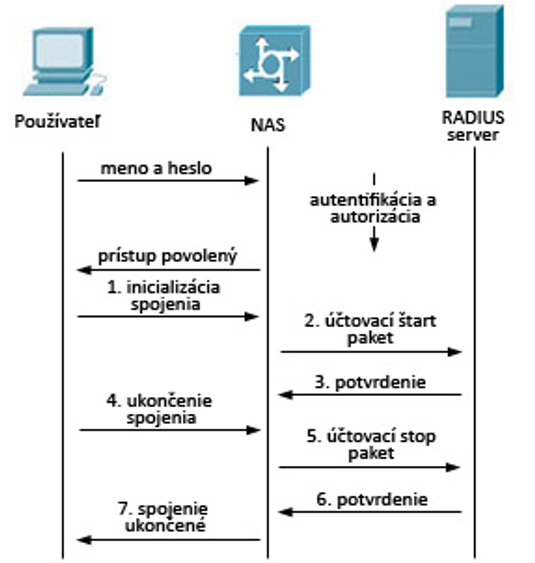
\includegraphics[width=0.6\linewidth]{obrazky/test_picture}
	\caption{Testovací obrázok}
	\label{fig:testpicture}
	\smallskip
	{\footnotesize Zdroj: vlastné spracovanie}
\end{figure}

\subsection{Tabuľky}

V tabuľke~\ref{tab:si_units} sú uvedené základné veličiny v elektronike.

\begin{table}[htbp] 
	\centering 
	\caption{Základné veličiny v elektronike}
	\label{tab:si_units} 
	
	% X - obsah stĺpca zarovnaný doľava
	% c - obsah stĺpca zarovnaný na stred
	\begin{tabularx}{0.8\linewidth}{X X c}
		\toprule
		\textbf{Veličina} & \textbf{Jednotka} & \textbf{Symbol} \\
		\midrule
		
		% --- Nadpis bloku 1 ---
		\multicolumn{3}{c}{\textbf{Technický blok 1}} \\
		\addlinespace[2pt]
		
		% --- Blok 1 ---
		\glsentrydesc{sym:U} & \glsentryuserii{sym:U} [\glsentryuseri{sym:U}] & \gls{sym:U} \\
		\glsentrydesc{sym:R} & \glsentryuserii{sym:R} [\glsentryuseri{sym:R}] & \gls{sym:R} \\
		\glsentrydesc{sym:I} & \glsentryuserii{sym:I} [\glsentryuseri{sym:I}] & \gls{sym:I} \\
		
		\midrule % --- Oddelenie blokov ---
		
		% --- Nadpis bloku 2 ---
		\multicolumn{3}{c}{\textbf{Technický blok 2}} \\
		\addlinespace[2pt]
		
		% --- Blok 2 ---
		\glsentrydesc{sym:U} & \glsentryuserii{sym:U} [\glsentryuseri{sym:U}] & \gls{sym:U} \\
		\glsentrydesc{sym:R} & \glsentryuserii{sym:R} [\glsentryuseri{sym:R}] & \gls{sym:R} \\
		\glsentrydesc{sym:I} & \glsentryuserii{sym:I} [\glsentryuseri{sym:I}] & \gls{sym:I} \\
		
		\bottomrule
	\end{tabularx}
	
	\smallskip
	\begin{center}
		{\footnotesize  Zdroj: vlastné spracovanie}
	\end{center}
\end{table}

\subsection{Rovnice}

Ohmov zákon vyjadruje vzťah medzi elektrickým napätím, elektrickým prúdom a elektrickým odporom:

\begin{equation} 
	\gls{sym:U} = \gls{sym:R} \cdot \gls{sym:I} 
	\label{eq:ohm} 
\end{equation} 

kde je

\begin{description}
	\item[\gls{sym:U}] \glsentrydesc{sym:U} [\glsentryuseri{sym:U}],
	\item[\gls{sym:R}] \glsentrydesc{sym:R} [\glsentryuseri{sym:R}],
	\item[\gls{sym:I}] \glsentrydesc{sym:I} [\glsentryuseri{sym:I}].
\end{description}


Ako je uvedené vo vzťahu~(\ref{eq:ohm}), elektrické napätie je priamo úmerné elektrickému prúdu.

\subsection{Skratky, citovanie použitej literatúry a jednotky}

\gls{bms} sú nevyhnutné pre elektrické vozidlá. \gls{cpu} spracúva inštrukcie v asembleri \cite{nuclear_fission_uranium_235, JAYABAL2024103121}.

Pri práci s jednotkami sa využíva balík \texttt{siunitx}, ktorý generuje jednotky nasledovne: \SI{4.00}{\celsius}, \SI{26.4}{\centi\metre}, \SI{0.322}{\milli\watt\per\cubic\centi\metre}, \SI{1}{\percent}, \SI{}{\celsius}.